\begin{abstract}
PHASE-TTC estimates signed time-to-contact (TTC) from synchronized events, RGB frames, and object regions supplied by the GarlTTC benchmark. The original event--RGB system obtained 35.80 Overall Motion-in-Depth (MiD) with zero scorer-defined failures on 6,762 private-test tokens, against 45.03 for the documented Garl-TTC reference. A second, pre-registered submission retained the RGB branch, added 600\,ms of causal box-expansion history from the supplied regions, and removed event inputs. It obtained 23.47 Overall MiD with zero scorer-defined failures. The comparison with Garl-TTC changes temporal support and learned components, while the second submission changes modality and measurement access. Equal-capacity EvTTC readout controls found no resolved benefit from event access or phase parameterization. On TRAIN40 folds, events improve a geometry-augmented head by 0.55 MiD [0.26, 0.88], within the pre-registered one-point simplification margin. The private result supports a benchmark-specific attribution to supplied-region history rather than a general claim for or against event sensing. A five-second replay returned all 250 outputs with a 29.14\,ms response p95, above a 20\,ms deadline. In a later 72-pass study, the two-packet policy delivered 9.6\% of offered PHASE outputs; a 64-packet queue delivered every output with per-scene response p95 values of 104--227\,ms. The evaluated chain excludes autonomous detection and calibrated collision risk.
\end{abstract}

\begin{table}[htbp]
\centering\footnotesize
\begin{tabularx}{\linewidth}{@{}p{.17\linewidth}p{.13\linewidth}p{.17\linewidth}Xp{.08\linewidth}@{}}
\toprule
Entry and date & Sensor inputs & Supplied-region and temporal support & Overall / bands c, s, l, n & Failure \\
\midrule
Garl-TTC reference\\28 Jun 2026 & Events + RGB & Regions; two observations 0.1 s apart & 45.03 / 53.13, 37.58, 40.61, 31.29 & 0\% \\
PHASE-TTC original\\28 Oct 2026 & Events + RGB & Regions; up to 650 ms history & 35.80 / 43.52, 28.26, 25.72, 29.93 & 0\% \\
PHASE-TTC-Geo\\18 Nov 2026 & RGB; no event input & Regions; 600 ms box history & 23.47 / 24.37, 23.95, 22.89, 18.13 & 0\% \\
\bottomrule
\end{tabularx}

\caption{Official GarlTTC Test scores on 6,762 tokens. Failure denotes the scorer's invalid-output rule. The rows use different models and temporal support.}
\label{tab:short-official}
\end{table}

\section{Related work}

\paragraph{Expansion and frame-based TTC.} TTC can be recovered from the ratio between apparent size and its temporal derivative under constant relative velocity \citep{lee1976}. Direct brightness-derivative methods extend that idea to image measurements under stronger surface and motion assumptions \citep{horn2007}. Learned monocular systems estimate optical expansion \citep{yang2020expansion}, classify whether contact falls inside time thresholds \citep{badki2021bittc}, or search for scale changes with correlation volumes \citep{ling2023tpcv,ling2024scaleflowpp}. TSTTC supplies a large frame-only driving benchmark for object-level TTC \citep{shi2023tsttc}. These methods motivate our supplied-box expansion control, but we do not evaluate them under one common training and test protocol.

\paragraph{Event-based TTC.} Event cameras record asynchronous brightness changes along moving contours. Classical TTC methods estimate flow divergence \citep{clady2014}, maximize contrast under scaling or motion models \citep{gallego2018cmax,mcleod2022}, or fit geometric motion to spatio-temporal events \citep{eventaided}. Learned event systems encode streams as voxel grids or learned tensors before applying spatial backbones \citep{zhu2019voxel,gehrig2019est}; E-RAFT uses correlation for event optical flow \citep{gehrig2021eraft}. These approaches can observe motion between RGB frames, but their inputs, object identity assumptions, and temporal windows differ.

\paragraph{Datasets and the principal comparator.} EvTTC provides synchronized event, RGB, box, and TTC data for driving scenarios \citep{evttc}. The eAP work defines the logarithmic MiD coordinate and introduces early and late event--RGB Garl models \citep{eap}. Its GarlTTC server supplies the private evaluation used here \citep{codabench2026,garlscorer2026}. FCWD comes from the event-aided TTC study and contains three approach recordings used in our later failure analysis \citep{eventaided}. We treat EvTTC and FCWD as development evidence because the project inspected their labels and reused them when designing controls.

\paragraph{Recent full-frame event inference.} REACT maintains a spiking state-space representation over full-frame events and reports 9.59\% RTE and 4.6\,ms on EvTTC under its own positive-TTC protocol \citep{react2026}. It does not require supplied object boxes. Its metric reduction, cohort, hardware, integration window, and timing boundary differ from the four-band private test and our queued service clock. We cite it as a relevant box-free event system rather than order its numbers against Table~\ref{tab:short-official}.

PHASE-TTC occupies a narrower position. It exposes named phase, timing, and support measurements from separately fitted RGB and event branches, then corrects an RGB anchor. The first submission evaluates that complete system. The second tests a different measurement source, causal history of supplied regions, while retaining the RGB branch. Matched controls below ask which part of those interfaces contributes within fixed development populations.

\section{Problem and evaluated systems}

TTC depends on the change in apparent scale, not scale alone. PHASE-TTC estimates motion separately in RGB and event observations, maps both branches to a signed phase coordinate, and uses a 1,955-parameter residual head to correct an RGB anchor. The original nine-component chain retains up to 650\,ms of causal history. Every benchmark query includes an object region; no autonomous detector is evaluated.

The project produced two private-test submissions. The original submission evaluates the complete event--RGB chain. The second retains the RGB estimates, appends causal slopes of supplied-box width, height, and area, uses the benchmark's band-weighted loss, and removes event inputs. We report both because the change tests whether the first result came from multimodal fusion or from motion information already present in the supplied regions.

\begin{figure}[htbp]
\centering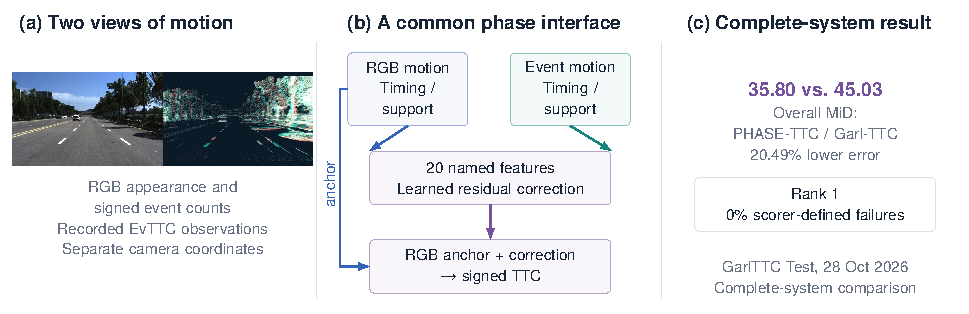
\includegraphics[width=\linewidth]{figures/publication_teaser.pdf}
\caption{The teaser records the original 35.80 system result. The second submission adds causal expansion of the supplied regions, omits event inputs, and obtains the 23.47 result in Table~\ref{tab:short-official}.}
\label{fig:short-overview}
\end{figure}

\subsection{Original phase-fusion chain}

Each modality has two motion producers. One follows a transport-trained route and one uses a coarse-to-fine route; a pairwise readout converts their fields into a signed phase estimate. A temporal refiner then summarizes the retained observations. These components have separate RGB and event weights. The fusion head never receives their hidden feature maps. It receives ten named values per modality: raw phase location, emitted point phase, three expert phases, four timing fields, and valid-history fraction. This interface avoids assuming that hidden coordinates from separately trained branches align.

For reference interval $d_0=0.1$\,s, the shared phase coordinate is
\begin{equation}
 \phi(T)=-\log\left(1-\frac{d_0}{T}\right).
\end{equation}
Positive phase denotes approach and negative phase denotes recession. Large TTC values lie near zero phase, while the sensitivity rises near the positive boundary $T=d_0$. The fusion input scales the first five phase-valued fields of each modality by $1/0.03$ and retains timing and support in their native units. A two-layer width-32 MLP predicts a residual around the RGB phase and two interval-width corrections. The factor 0.03 scales the residual; it does not bound it. Output conversion clips phase to its supported domain and limits TTC magnitude to 60\,s near zero expansion. The reported widths are empirical phase intervals, not calibrated collision probabilities.

\begin{figure}[htbp]
\centering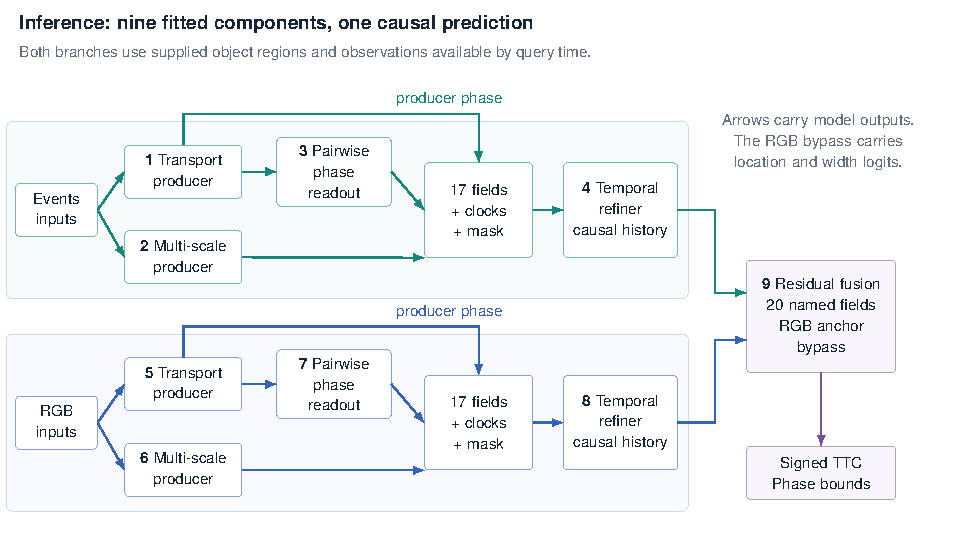
\includegraphics[width=\linewidth]{figures/publication_architecture.pdf}
\caption{Original nine-component chain. RGB and event producers have separate weights; only named estimates, timing, and support reach the fusion head.}
\label{fig:short-architecture}
\end{figure}

Object regions define a common square coordinate frame across each endpoint pair. Independent tight crops would remove part of the expansion signal. RGB processing uses the latest causal frame; event processing accumulates causal prefixes. The original chain retains at most eight temporal observations within 650\,ms. Aliases in the submission package reuse a physical query and do not trigger extra inference.

The geometry submission adds ten features computed only from preceding supplied regions: robust slopes and support diagnostics derived from width, height, and square-root area. It keeps the RGB branch and discards the original event fields. This is a new head, distinct from the three-router PHASE-TTC-Adapt model distributed on the Hub. The scored PHASE-TTC-Geo package is bound to submission 1058935 and is not either published Hub checkpoint.

\section{Metric, submissions, and comparator scope}

The scorer uses
\begin{equation}
 \mathrm{MiD}(\widehat T,T)=10^4\left|\log\left(1-\frac{0.1}{T}\right)
 -\log\left(1-\frac{0.1}{\widehat T}\right)\right|
\end{equation}
and combines the crucial, small, large, and negative TTC bands with weights 0.5, 0.3, 0.1, and 0.1. Overall MiD is therefore a phase-coordinate error with asymmetric band weights, not TTC error in seconds.

The original submission is 20.49\% below the reference. PHASE-TTC has longer temporal support and different upstream models, so the official comparison establishes a complete-system result. It does not isolate fusion. The second submission is 34\% below the original and 48\% below the reference. Its crucial-band reduction from 43.52 to 24.37 contributes 9.58 of the 12.33 Overall points because that band carries half the score. The result is not uniform across TTC regimes. The public leaderboard and scorer records provide the official identity, population, bands, and failure rule \citep{codabench2026,garlscorer2026}.

Garl-TTC's official row comes from the leaderboard. Separate local controls use released checkpoints: the adapter selects two causal RGB endpoints nearest 100\,ms apart, constructs a polarity-agnostic 20-plane event volume with at most 100\,ms support at each endpoint, forms a common square crop from supplied regions, and converts predicted height ratio using the measured endpoint separation. These development controls do not reproduce the official row. Their local preprocessing and timing implementation remain part of their measured result.

\section{Training, selection, and exposure}

The original head uses grouped out-of-fold TRAIN40 features. A 20-field descriptor contains five phase values, four timing fields, and one support value per modality. Exact-constancy counts are 4 of 20 fields in TRAIN40, 6 in the private-test inputs, and 9 in EvTTC. Two phase-field pairs are also nearly identical on EvTTC. The event history uses a 50\,ms fitting grid but a 100\,ms inference grid. Matching the grid after submission did not recover an event benefit on the inspected EvTTC cohort.

The geometry study refits heads under five sequence-disjoint blocks and three seeds. A fixed rule selects the lowest band-weighted Overall MiD among variants whose recording-bootstrap interval against the released recipe excludes zero, with ties within one point resolved toward fewer inputs. The rule selects RGB plus box expansion without event fields. A receipt binds the code, seed, package, and hypothesis before upload.

The original training chain also uses grouped out-of-fold construction. Producer and context models generate features only for groups excluded from their own fit before the fusion head sees those rows. Final deployed producers then refit on the complete training population. This procedure separates rows during head fitting but does not create an independent acquisition: model selection, representation choices, and later diagnostics repeatedly inspect the same sequence families.

Three head seeds measure optimization variation conditional on shared upstream features. They do not represent three independent encoders or datasets. Confidence intervals resample complete recordings or sequence groups rather than adjacent windows. This preserves within-recording dependence, but intervals on inspected recordings remain conditional on development exposure. No multiplicity correction is applied.

\begin{figure}[htbp]
\centering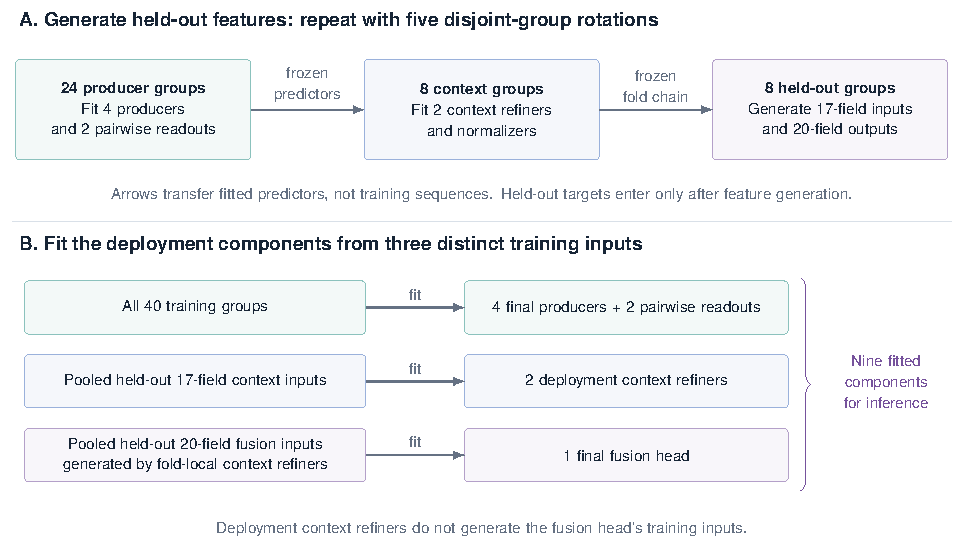
\includegraphics[width=\linewidth]{figures/publication_oof.pdf}
\caption{Grouped feature construction for the original head. Out-of-fold rows support head fitting; final inference uses producers refitted on the complete training population.}
\label{fig:short-oof}
\end{figure}

The adaptation records enumerate 21, 117, 312, and 48 fits in four named campaigns, or 498 fits within those campaigns. Other development work is inventoried separately because records may overlap. Intervals on those recordings describe an inspected cohort. The original private score was unavailable when its recipe was selected. The second recipe was selected after the first score existed, so the two submissions are sequential uses of one server rather than independent datasets.

\section{Attribution controls}

Matched readout experiments keep upstream features and histories fixed. Three seeds of equally sized heads compare real-event and zero-event inputs, phase and inverse-TTC coordinates, and an RGB anchor. The mean transfer MAE is 0.847\,s for real-event phase heads and 0.838\,s for zero-event heads; their paired recording-bootstrap interval includes zero. Phase and inverse-TTC heads also have unresolved differences. The refitted phase heads are not separated from RGB alone. These controls do not support attribution of the original private gain to event access or the phase coordinate.

\begin{table}[htbp]
\centering\footnotesize
\begin{tabular}{lrr}
\toprule
Readout & MAE (s) & Relative error (\%) \\
\midrule
Phase correction, real events & $0.847\pm0.038$ & $30.92\pm2.05$ \\
Phase correction, zero events & $0.838\pm0.021$ & $29.12\pm1.16$ \\
Inverse-TTC correction, real events & $0.847\pm0.041$ & $30.80\pm2.14$ \\
Source-calibrated scalar phase mixture & 0.996 & 36.23 \\
\bottomrule
\end{tabular}

\caption{Equal-capacity readouts on fixed final-model features and histories. Results use development-exposed EvTTC recordings; lower MAE is better.}
\label{tab:short-heads}
\end{table}

Simple mixtures provide a second reference. Equal phase and inverse-TTC mixtures are worse than the fitted heads. A one-parameter source-calibrated phase mixture narrows the difference, and its remaining margin depends largely on one recording. This comparison shows that a learned correction can fit branch reliability on the inspected cohort; it does not identify which sensor supplies new causal information.

On TRAIN40 folds, box expansion lowers the refitted released head from 85.17 to 41.96 Overall MiD, and band weighting without event inputs lowers it to 41.27. Fold levels are not comparable with server levels. A box-only head obtains 46.09, so RGB estimates account for 4.82 fold points beyond supplied-box history. Replacing the RGB fields with the released Garl event-model prediction yields 40.57; the interval for its 0.70-point difference from the selected head includes zero, and the Garl predictions are in-sample on those folds.

\begin{table}[htbp]
\centering\footnotesize
\begin{tabular}{lrrrr}
\toprule
Readout & Inputs & Overall MiD & Crucial & $\Delta$ vs released recipe \\
\midrule
Released recipe, refit in grouped folds & 20 & $85.17\pm0.04$ & 132.4 & --- \\
\quad with band-weighted loss & 20 & $78.01\pm0.10$ & 109.5 & -7.16 $[-9.53,-4.82]$ \\
\quad with box-expansion inputs & 30 & $41.96\pm0.42$ & 56.6 & -43.21 $[-52.64,-34.09]$ \\
\quad with both & 30 & $40.72\pm0.20$ & 50.9 & -44.46 $[-53.91,-35.19]$ \\
RGB fields, box expansion, band loss (selected) & 20 & $41.27\pm0.29$ & 51.1 & -43.90 $[-53.38,-34.55]$ \\
Box expansion only, learned & 10 & $46.09\pm0.10$ & 53.3 & -39.09 $[-49.84,-28.57]$ \\
Box expansion only, fixed estimator & --- & $74.46$ & 100.2 & -10.71 $[-21.22,-0.49]$ \\
Best constant & --- & $198.08$ & 187.9 & +112.91 $[+105.37,+120.24]$ \\
\bottomrule
\end{tabular}

\caption{Geometry and branch inputs on TRAIN40 development folds. Levels cannot be compared directly with private-test scores.}
\label{tab:short-geometry}
\end{table}

The table separates a fixed geometric estimator from learned heads. The fixed estimator performs poorly because clipped boxes, lateral motion, and noisy slopes violate its expansion model. Learned heads can reject or correct those estimates using branch predictions and quality fields. The selected no-event head wins under the pre-registered rule, although the event-augmented geometry head is about half a fold point lower. The tie rule prefers fewer inputs within one point. The second private submission validates the selected recipe's direction under this benchmark; it does not convert the fold difference between event and no-event heads into a private causal comparison.

Follow-up FCWD controls expose a boundary of box geometry. Once an object fills the frame, clipped box edges stop expanding. A direct event-derived content-scale estimate improves that saturated stratum on three development-exposed sequences, but this arm was not scored on the private server. The second submission therefore supports supplied-region history under the benchmark contract, while the event-derived measurement remains relevant where that contract loses geometric information.

\section{Runtime and limitations}

Runtime separates service time from scheduled-arrival response and delivery coverage. The historical five-second replay on a laptop GPU returns all 250 outputs with numerical parity. Response p95 is 29.14\,ms, and 201 outputs meet or exceed the 20\,ms deadline. A later study runs 72 fresh-process passes across six scenes. With a two-packet queue, one of 24 PHASE replays completes and 9.6\% of offered outputs are delivered. With a 64-packet queue, every PHASE output is delivered, with per-scene response p95 values of 104--227\,ms. The small-queue failure occurs near startup; its cause was not isolated. Larger queues trade drops for delayed responses.

\begin{figure}[htbp]
\centering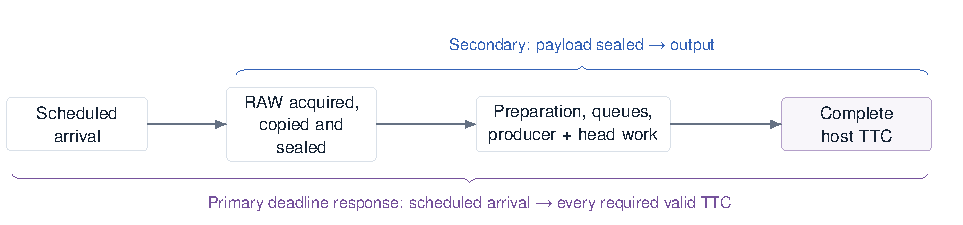
\includegraphics[width=\linewidth]{figures/publication_runtime_clock.pdf}
\caption{The service study keeps acquisition, queueing, preparation, model execution, and delivery clocks distinct. A low model-forward time cannot establish deadline coverage.}
\label{fig:short-runtime-clock}
\end{figure}

The response clock begins at scheduled packet availability and ends when a host-visible TTC is returned. Model loading, disk access, and the initial synthetic shape prime precede measured arrivals. Preparation triggered by a request remains inside response time. The service clock begins after dequeue, so it excludes prior waiting but includes input construction and synchronization. Coverage counts every offered output, including drops and history-gap refusals. Percentiles over delivered outputs are reported with delivered fraction because discarding missed requests can make a failing queue appear fast.

The local Garl service constructs event volumes on a CPU cache-miss path and hashes prepared inputs inside each measured call. PHASE advances event prefixes on the GPU. The timing comparison measures those implementations; it does not give a hardware-independent architectural ranking. The complete learned PHASE variants miss 20\,ms under the tested clocks. An isolated CPU box-only head meets the deadline on 600 queries, but it is not the scored geometry system.

The 600-query variant timing control is an isolated, host-paced replay over preloaded supplied-box cells. It is not a sustained 60-second sensor service, does not include a detector, and does not validate a separate availability clock. The box-only median of 0.39\,ms and maximum of 1.63\,ms describe that narrow computation. The scored geometry variant still executes the RGB branch; with cached earlier observations it has a 28.8\,ms median and 36.2\,ms p95 in this control. Recomputing its history takes longer. These values cannot be substituted for the queued six-scene service response.

The benchmark supplies regions without detector delay, and the private labels permit two server evaluations rather than a new acquisition. The eAP description derives annotations and TTC truth from 3D scene information, while its released builder passes stored annotation boxes to the model \citep{eap}. A label-free audit projects the eight 3D cuboid corners and reproduces the four TRAIN40 box edges after clipping and integer truncation for all 88,744 queries. It reads no TTC or private-test value and does not establish Test12 box provenance. The result makes an independent detector with measured delay and jitter necessary before transferring the geometry result to camera operation. Secondary cohorts were inspected during development. Historical replay changes 504 of 5,805 original physical-query predictions beyond the old tolerance, although the mean bound in benchmark coordinates is 0.010 MiD without private labels. The archived packages and scoring records remain the evidence for the official results. Synchronized unused event--RGB recordings, calibrated risk, and sustained multi-object service remain open.

\section{Conclusion}

The original event--RGB system obtains 35.80 Overall MiD. Matched controls do not isolate a gain from events or phase fusion. A pre-registered RGB-plus-box-history variant obtains 23.47 without event inputs. TRAIN40 controls assign the largest measured development gain to causal history of the supplied regions; the private result confirms the selected recipe, not that causal attribution. REACT addresses a box-free full-frame regime. Our event-derived content-scale control instead operates inside supplied boxes and remains relevant when their edges saturate. The tested learned services do not meet a continuous 20\,ms response contract.
